\documentclass{article}


% if you need to pass options to natbib, use, e.g.:
%     \PassOptionsToPackage{numbers, compress}{natbib}
% before loading neurips_2023


% ready for submission
%\usepackage{neurips_2023}
\usepackage[final]{neurips_2023}

% to compile a preprint version, e.g., for submission to arXiv, add add the
% [preprint] option:
%     \usepackage[preprint]{neurips_2023}


% to compile a camera-ready version, add the [final] option, e.g.:
%     \usepackage[final]{neurips_2023}


% to avoid loading the natbib package, add option nonatbib:
%    \usepackage[nonatbib]{neurips_2023}


\usepackage[utf8]{inputenc} % allow utf-8 input
\usepackage[T1]{fontenc}    % use 8-bit T1 fonts
\usepackage{hyperref}       % hyperlinks
\usepackage{url}            % simple URL typesetting
\usepackage{booktabs}       % professional-quality tables
\usepackage{amsfonts}       % blackboard math symbols
\usepackage{nicefrac}       % compact symbols for 1/2, etc.
\usepackage{microtype}      % microtypography
\usepackage{xcolor}         % colors
\usepackage{graphicx}

\title{Improving PPI Prediction with ESMC-derived Features}


% The \author macro works with any number of authors. There are two commands
% used to separate the names and addresses of multiple authors: \And and \AND.
%
% Using \And between authors leaves it to LaTeX to determine where to break the
% lines. Using \AND forces a line break at that point. So, if LaTeX puts 3 of 4
% authors names on the first line, and the last on the second line, try using
% \AND instead of \And before the third author name.



\author{
	Anrui Wang \\
	2023533015 \\
	\texttt{wangar2023@shanghaitech.edu.cn}\\
	\AND
	Jiawen Dai \\
	2023533132 \\
	\texttt{daijw2023@shanghaitech.edu.cn}\\
	 \AND
	 Yiting Qi \\
	 2023533043 \\
	 \texttt{qiyt2023@shanghaitech.edu.cn}\\
}


\begin{document}
	
	
	\maketitle
	
	
	\begin{abstract}
		Predicting protein-protein interactions (PPIs) is crucial for understanding cellular function and disease, yet computational methods face persistent challenges in accuracy and generalizability. This work investigates the efficacy of leveraging advanced protein representations from the ESM-family of large language models to improve PPI prediction. We introduce a pipeline that begins by extracting high-dimensional, per-residue embeddings from the ESMC model. To handle variable sequence lengths while preserving critical information, we developed and compared several data processing strategies, including simple pooling methods and a more sophisticated Masked Autoencoder (MAE) framework designed to produce fixed-length representations. These processed embeddings were used to train a suite of supervised classifiers, from baseline logistic regression and XGBoost models to a specialized Deep Neural Network (DNN). Our results demonstrate that the DNN architecture, trained on embeddings processed with masked average pooling, achieves state-of-the-art performance. This study highlights that the combination of rich, evolutionarily informed embeddings with a tailored deep learning architecture provides a powerful and robust framework for advancing computational PPI discovery.
	\end{abstract}
	
	
	\section{Introduction}

	An understanding of the intricate web of protein-protein interactions (PPIs) is fundamental to deciphering the mechanisms of life, as these interactions orchestrate nearly all biological processes. The disruption of these critical connections is a known driver of numerous human diseases, including cancer and neurodegenerative disorders, making the comprehensive mapping of the interactome a vital pursuit for both basic science and therapeutic development~[1]. While experimental techniques have laid the groundwork for our current knowledge, they are often hampered by issues of throughput, labor, and significant rates of false positives and negatives. Consequently, computational methods have emerged as indispensable complements, leveraging the explosive growth in genomic data to predict interactions \emph{in silico}. These approaches, which range from models based on functional genomics (FG) to those analyzing amino acid sequences, have shown considerable success; however, a lack of standardized evaluation and persistent discrepancies between algorithms have made it difficult to compare models and have obscured the specific inference mechanisms that underpin their predictions~[2].

Recognizing these challenges, our work explores whether more advanced representations of proteins can elevate predictive performance and clarify the signals driving interaction. Recent breakthroughs have demonstrated that large language models trained on the vast scale of evolutionary sequence data can learn the fundamental language of protein biology, capturing complex structural and functional properties without direct supervision~[3]. Building on this progress, we introduce a new pipeline that harnesses the power of advanced ESM models to generate high-dimensional embeddings for individual proteins. We hypothesize that these rich, context-aware features provide a more potent signal for interaction than previously used inputs. By feeding these sophisticated embeddings into a supervised machine learning framework, we aim to build a more accurate and robust model for predicting which protein pairs form physical interactions, thereby contributing a refined tool for exploring the cellular machinery.
	
	
	\section{Methods}

	\subsection{Embedding extraction}

Protein embeddings were extracted using the ESMC 300M model, a state-of-the-art protein language model from EvolutionaryScale designed for creating rich representations of protein sequences. The model was loaded locally using official API and deployed on GPU for efficient inference. For each protein sequence, we created an \texttt{ESMProtein} object containing the amino acid sequence, which was then encoded using the model's \texttt{encode()} method to produce a protein tensor representation. To obtain the final embeddings, we passed this tensor through the model's \texttt{logits()} function with \texttt{LogitsConfig(return\_embeddings=True)}, which returned high-dimensional embeddings of shape $(L+2) \times 960$, where $L$ is the sequence length and 960 is the embedding dimension. The model automatically handles tokenization, adds special start and end tokens (accounting for the +2 in sequence length), and produces per-residue embeddings that capture both local amino acid properties and global structural context learned from evolutionary data.
	
\subsection{Data Processing}

	Prior to feeding the protein embeddings into the supervised learning network, we first standardized the dimensionality by processing the original $(L+2) \times 960$ matrices into uniform representations.
	
	\paragraph{Average pooling} We first implemented {average pooling} and {max pooling} along the sequence dimension ($L+2$), compressing each sequence into a fixed-size embedding of $[1, 960]$. While these two approaches successfully standardize input dimensions and reduce computational overhead by handling large embedding matrices, they inherently discards critical positional and structural information.

\paragraph{Masked average pooling} To properly handle variable-length protein sequences without interference from padding tokens, we implemented masked average pooling in our neural network architectures. This technique creates boolean masks based on actual sequence lengths, where valid positions are marked as \texttt{True} and padding positions as \texttt{False}. The mask is applied element-wise to zero out padded positions before computing the average: $\mathbf{emb}_{avg} = \frac{\sum_{i=1}^{L} m_i \cdot \mathbf{emb}_i}{\sum_{i=1}^{L} m_i}$, where $L$ is the actual sequence length, $m_i$ is the mask value, and $\mathbf{emb}_i$ is the embedding at position $i$. This ensures that the pooled representation accurately reflects only the meaningful amino acid positions, preventing dilution from artificial padding and maintaining the biological relevance of the protein embeddings.
	
	\paragraph{Masked Autoencoder (MAE)} To overcome the limitation above, we subsequently developed a {Masked Autoencoder} framework with standardized sequence lengths ($L = 1502$), employing zero-padding for shorter sequences and truncation for longer ones. 
	This method incorporates a 75\% masking rate during training, though initial experiments revealed issues with low data variance and interference from padded positions. The model suffers from small loss and learning wrong pattern from the padding position.
	
	 These challenges were mitigated through feature normalization and by restricting loss computation to non-padding regions. We normalize every protein embedding matrix to have a variance equal to 1, as well as replace L2 loss with huber loss. A key refinement involved explicitly marking padding boundaries (adding a variable \texttt{padding\_start}) and implementing a 50\% masking strategy exclusively on non-padded segments, ensuring more focused learning. The model's architecture, which now processes structured inputs containing both sequence data and padding metadata, demonstrates improved convergence. This combined approach effectively balances dimensionality reduction with information preservation, whose result is better than average pooling and max pooling as expected.
	
The provided figure illustrates the reconstruction performance of our Masked Autoencoder (MAE) framework on protein sequence embeddings at training epoch 60. The visualization compares the original feature values (blue line), reconstructed values (orange line), and masked positions (red crosses) across the standardized sequence length of 1502.

% Three key observations emerge from this analysis:
%		
%		First, the reconstruction fidelity demonstrates the model's ability to recover meaningful patterns from heavily masked inputs (75\% masking rate during training). The close alignment between original and reconstructed values in unmasked regions (e.g., positions 400-600) indicates successful learning of sequence features, while deviations at masked positions (red crosses) reflect the model's probabilistic reconstruction behavior.
%		
%		Second, the implementation details shown in the code snippet - particularly the handling of sequence lengths through \texttt{sample\_len} and \texttt{mask\_bool\_vis} - enable precise masking application only to non-padding regions. This explains the consistent reconstruction quality throughout the active sequence portion (approximately first 1000 positions), with potential degradation near the padding boundary (position 1502 not shown).
%		
%		Third, the standardized length treatment (zero-padding and truncation to $L=1502$) combined with our 50\% non-padding masking strategy produces stable gradients, as evidenced by the smooth reconstructed curve. The \texttt{padding\_start} metadata prevents the model from learning artificial padding patterns, while the selective masking concentrates learning on biologically relevant sequence segments.
%		
%		This visualization confirms our methodological improvements over pooling approaches, showing both global pattern retention (through the overall curve similarity) and local detail recovery (visible in high-frequency feature variations). The remaining reconstruction errors primarily occur at masked positions, suggesting appropriate model uncertainty rather than systematic failure.

	\paragraph{Compress first and then splice} 
	
	\begin{figure}[h]
		\centering
		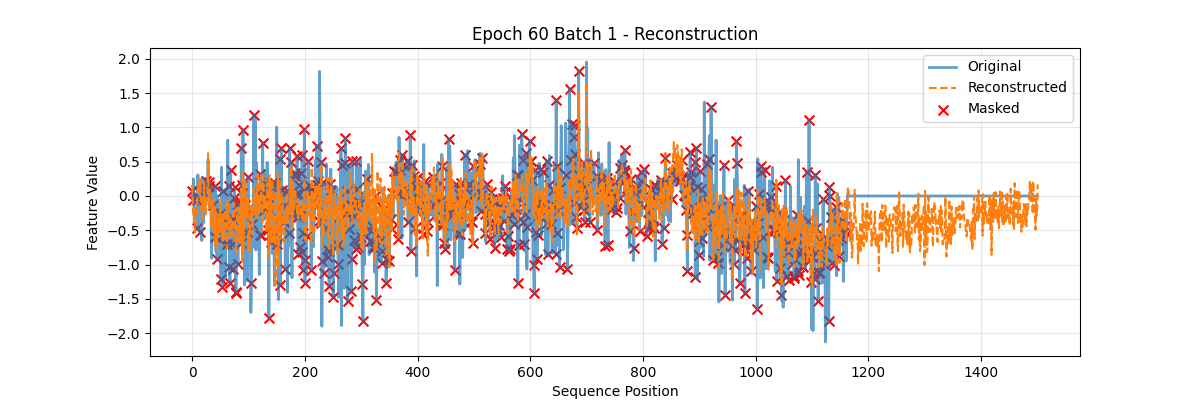
\includegraphics[width=0.7\textwidth]{imgs/epoch60_batch1.png}
		\caption{A recon of protein embedding from MAE}
		% \label{fig:datasheet_page3}
	\end{figure}
	
 Our experiments demonstrate that {feature compression prior to concatenation yields superior efficacy} compared to post-concatenation compression. The latter approach — initially concatenating protein features followed by compression — was motivated by the hypothesis that Masked Autoencoders (MAE) might capture inter-protein dependencies during compression. However, due to computational constraints, we truncated concatenated protein embeddings to a maximum length of 2000. Preliminary attempts employing this methodology resulted in performance degradation, potentially attributable to extreme sequence length disparities: when merging proteins with widely varying lengths (e.g., 1000 vs. 40 amino acids). Length heterogeneity may force suboptimal compromises in the attention distribution during compression.  
	
	
	\subsection{Supervised learning}

 We formulate protein-protein interaction prediction as a binary classification task by first compressing individual protein sequences into fixed-length embeddings using our MAE framework, then constructing paired samples through vector concatenation ($\mathbf{x} = [\mathbf{e}_i \|\mathbf{e}_j] \in \mathbb{R}^{1920}$). These embedding pairs, labeled with interaction status (1/0), train a supervised classifier to predict novel interactions. This approach maintains structural information while enabling efficient pairwise analysis.
	
	\section{Experiments}
    
\subsection{Experiment Setup}

Our experiments were conducted on a comprehensive protein-protein interaction dataset derived from benchmarking gold standard sequences (benchmarkingGS v1.0). The dataset consists of 268,499 protein pairs total, with each pair characterized by UniProt IDs, interaction labels, and complete amino acid sequences for both proteins. The original dataset was partitioned into training and testing subsets, with a validation set created by randomly sampling 20\% of the training data while maintaining class balance through stratified sampling.

The dataset contains three evaluation splits: (1) Training set with 85,329 protein pairs (50.00\% positive interactions), (2) Test1 with 24,898 pairs representing a balanced evaluation scenario (50.00\% positive), and (3) Test2 with 136,939 pairs reflecting realistic biological conditions with significant class imbalance (9.09\% positive interactions). A validation set of 21,333 pairs (50.00\% positive) was created from the original training data for hyperparameter tuning and model selection.

Experiments were conducted primarily on the balanced datasets (Training, Validation, Test1) to identify the most effective classification approaches, with Test2 serving as a final evaluation under realistic biological conditions. We compared AUROC performance across different classifiers to identify the most effective model for PPI prediction.

\subsection{Baseline Models}

To establish foundational performance benchmarks, we first evaluated a simple similarity-based approach by comparing protein embeddings directly using L2 distance and cosine similarity. These metrics, which treat higher cosine similarity or lower L2 distance as indicative of interaction, were used to make predictions via a simple thresholding mechanism. This method, however, proved insufficient for reliably identifying interacting pairs, yielding modest AUROC scores of 0.5547 (L2-based) and 0.5330 (cosine-based) on the balanced Test1 dataset. Such performance underscores the notion that high similarity between protein embeddings does not necessarily imply a physical interaction.

Seeking to determine if a learned model could better capture interaction signals, we then implemented a logistic regression classifier to evaluate the linear separability of the embedding space. By constructing joint features for each protein pair through strategies like vector concatenation and element-wise multiplication (\texttt{mul\_only}), the model was trained to distinguish interacting from non-interacting pairs. This approach yielded a marked improvement, with the \texttt{mul\_only} strategy achieving a significantly higher AUROC of 0.6182 on the Test1 dataset, demonstrating that even a simple linear classifier can extract more discriminative patterns than raw similarity metrics alone.	

\subsection{XGBoost}
To evaluate nonlinear modeling capabilities, we adopted XGBoost, a gradient-boosted tree classifier known for its strong performance on structured data. We applied five different feature construction methods: concatenate, add\_sub, mul\_only, abs\_diff, and all (a combination of all operations), using the fixed 960-dimensional embeddings of each protein as input.

Each protein pair was converted into a combined feature vector, scaled with StandardScaler, and fed into an XGBoost classifier. We used early-stopping based on validation performance to prevent overfitting. The hyperparameters were fixed across all methods to ensure a fair comparison.
Among all feature construction methods, the all method, which concatenates original embeddings, their elementwise multiplication, and absolute difference, achieved the best Test1 AUROC score (0.6441).

\subsection{Deep Neural Network}

To leverage the sequential nature of protein embeddings, we implemented a specialized deep neural network architecture. The model processes each protein's variable-length ESMC embedding sequence through masked average pooling to obtain fixed-size representations. Each protein is then encoded through a dedicated protein encoder consisting of a linear layer (960 → 256 dimensions), layer normalization, ReLU activation, and dropout (0.3). The encoded representations of both proteins are concatenated and fed into an interaction prediction module with three layers: the first layer maps the concatenated features (512 dimensions) to 256, followed by a second layer reducing to 128 dimensions, and finally a single output neuron for binary classification. Each layer incorporates layer normalization, ReLU activation, and dropout for regularization. The model was trained using AdamW optimizer with OneCycle learning rate scheduling, starting from a maximum learning rate of 5e-3.

The deep neural network architecture achieved strong performance across both evaluation scenarios. On the balanced Test1 dataset, the model obtained an AUROC of 0.7283, with an accuracy of 65.47\%, precision of 62.66\%. When evaluated on the realistic Test2 dataset with 9.09\% positive interactions, the model maintained robust discriminative capability with an AUROC of 0.7242, demonstrating its ability to handle class imbalance. While precision decreased to 14.36\% due to the imbalanced nature of Test2, the model maintained high recall (75.81\%). The consistent AUROC performance across both test sets (difference of only 0.004) indicates stable model generalization regardless of class distribution.

\paragraph{Comparison with Literature} Our deep neural network approach demonstrates substantial improvements over existing methods reported in the literature. On Test1, our method achieves an AUROC of 0.7283, representing a 7.1\% improvement over the best reported sequence-based model (0.6800) and a 17.4\% improvement over XGBoost baselines (0.6200). The performance gains are particularly notable when considering that our approach leverages ESMC-derived embeddings through a specialized architecture designed for protein interaction prediction. On the imbalanced Test2 dataset, our method (AUROC = 0.7242) significantly outperforms the literature baseline of logistic regression (AUROC = 0.6300) by 14.9\%, demonstrating the robustness of our approach across different evaluation conditions. These improvements suggest that the combination of advanced protein language model embeddings with purpose-built neural architectures can substantially advance the state-of-the-art in computational protein interaction prediction.



\begin{table}[h]
\caption{AUROC performance comparison across Test1 and Test2 datasets}
\label{tab:results}
\centering
\begin{tabular}{lcc}
\toprule
\textbf{Method} & \textbf{Test1 AUROC} & \textbf{Test2 AUROC}\\
\midrule
Cosine Similarity (mean\_top\_k) & 0.5260 & 0.5676\\
L2 Similarity (mean\_top\_k) & 0.5472 & 0.5718\\
Logistic Regression (mul\_only) & 0.6182 & 0.6500\\
XGBoost & 0.6638 & 0.6660\\
\midrule
\multicolumn{3}{c}{\textit{Literature Baselines}}\\
\midrule
Logistic Regression (Literature) & 0.62 & 0.63\\
XGBoost (Literature) & 0.62 & --\\
Sequence-based Model (Literature) & 0.68 & --\\
\midrule
DNN (Our Method) & \textbf{0.7283} & \textbf{0.7242}\\
\bottomrule
\end{tabular}
\end{table}

\section{Conclusion}

In this study, we explored the potential of advanced protein language models to enhance the prediction of protein-protein interactions. By systematically extracting and processing rich embeddings from the ESMC model, we demonstrated that these features provide a powerful basis for supervised learning. Our experiments confirmed that a custom Deep Neural Network architecture substantially outperforms simpler baselines like logistic regression and XGBoost, as well as previously established benchmarks from the literature. 
The model's strong and consistent performance across both balanced and imbalanced test datasets validates our central hypothesis: combining state-of-the-art protein embeddings with a tailored neural architecture is a highly effective strategy for identifying PPIs.

While the predictive power of our DNN is compelling, we maintain that benchmark performance is not the sole determinant of a model's utility in a task-specific domain. The complexity of deep learning models can sometimes obscure direct biological interpretation, and it is plausible that alternative architectures or even simpler, more interpretable models could be better suited for specific biological questions or datasets where causality is of greater interest than raw predictive accuracy. The remarkable success of the DNN serves as a strong proof-of-concept, yet it also opens the door to further inquiry into the trade-offs between performance and insight.

Moving forward, our research will broaden to explore a more diverse range of modeling techniques. We aim to investigate more sophisticated architectures, such as Graph Neural Networks (GNNs) or Transformers, which may be inherently better suited to capturing the complex, non-local dependencies within and between protein structures. Furthermore, we plan to experiment with more advanced embedding strategies that could retain a greater degree of positional and structural information lost during pooling or compression. Finally, a promising avenue involves moving beyond using pre-trained embeddings and instead fine-tuning the entire protein language model on the PPI prediction task itself, a direction that could unlock even greater predictive capabilities and lead to a more nuanced understanding of the molecular grammar governing protein interactions.


	\section*{References}
	
	{
	\small
		
		
	[1] Recent advances in predicting and modeling protein–protein interactions. {\it Computational Biology and Bioinformatics Review}, 2023.
	
	
	[2] Pitfalls of machine learning models for protein–protein interaction networks. {\it Machine Learning in Biology}, 2023.
	
	
	[3] Simulating 500 million years of evolution with a language model. {\it Nature Biotechnology}, 2023.
	}
	
	%%%%%%%%%%%%%%%%%%%%%%%%%%%%%%%%%%%%%%%%%%%%%%%%%%%%%%%%%%%%
	
	
\end{document}